\documentclass[tikz]{standalone}

%%% Packages
\usepackage{tikz}
\usetikzlibrary{positioning, shapes, snakes}


%%%%%%%%%%%%%%%%%%%%%%%%%%%%%%%%%%%%%%%%%%%%%%%%%%%%%%%%%%%%%%%%%%%%%%%%%%%%%%%
\begin{document}

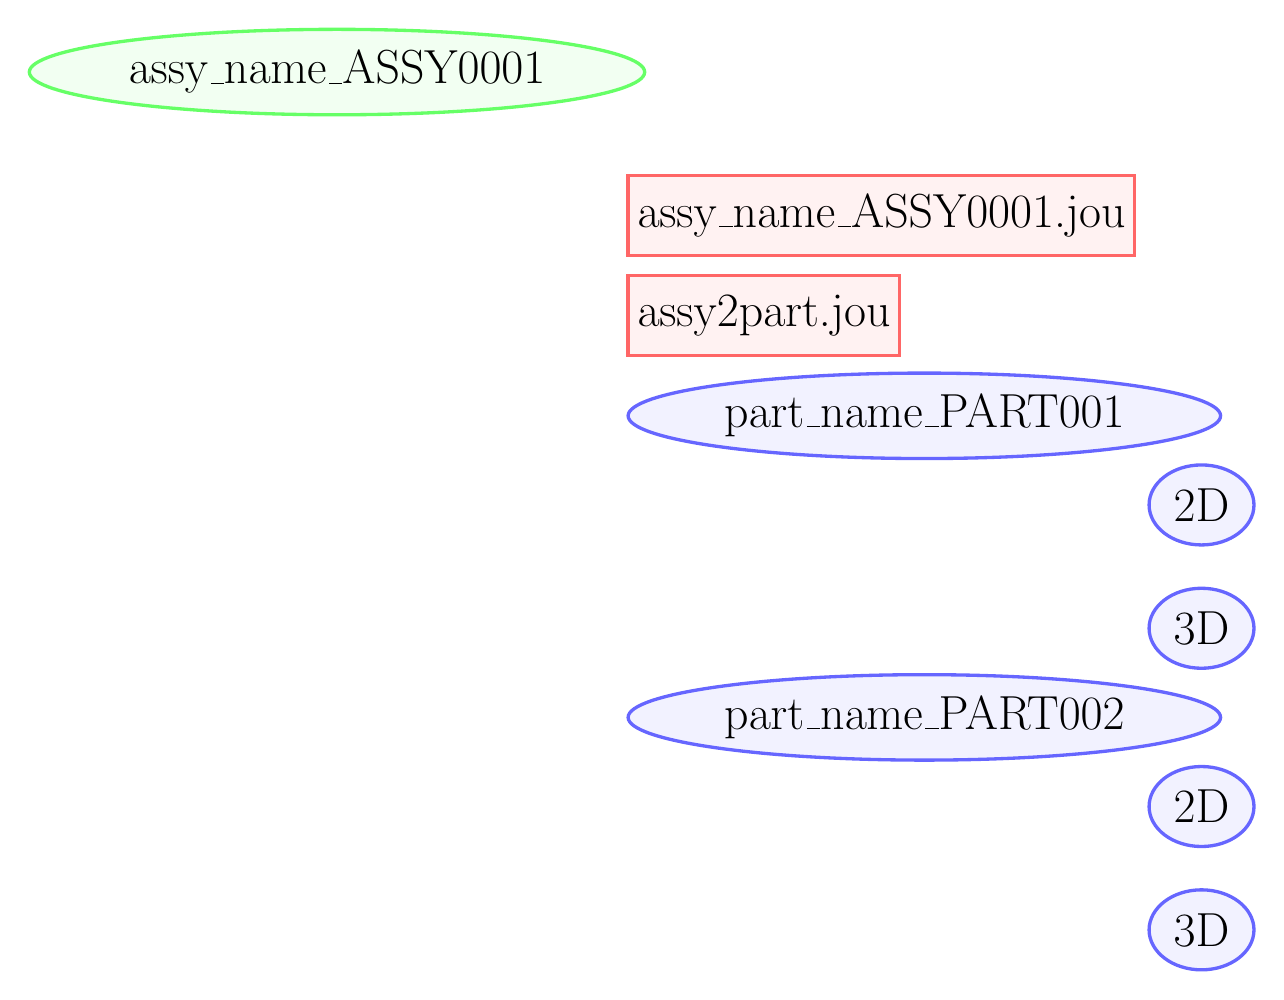
\begin{tikzpicture}[
  maindir/.style={ellipse, draw=green!60, fill=green!5, very thick, minimum size=0.4in},
  subdir/.style={ellipse, draw=blue!60, fill=blue!5, very thick, minimum size=0.4in},
  file/.style={rectangle, draw=red!60, fill=red!5, very thick, minimum size=0.4in},
  node distance=0.5in,
]

%%% Nodes
\node[maindir] (maindir) {\LARGE assy\_name\_ASSY0001};
\node[file] (assyjou) [draw, below right=of maindir] {\LARGE assy\_name\_ASSY0001.jou};
\node[file] (assy2part) [below=of assyjou.west, anchor=west] {\LARGE assy2part.jou};
\node[subdir] (partdir1) [below=of assy2part.west, anchor=west] {\LARGE part\_name\_PART001};
\begin{scope}[node distance=0.2in]
  \node[subdir] (dir2D1) [below right=of partdir1] {\LARGE 2D};
  \node[subdir] (dir3D1) [below=of dir2D1] {\LARGE 3D};
  \node[subdir] (partdir2) [below left=of dir3D1] {\LARGE part\_name\_PART002};
  \node[subdir] (dir2D2) [below right=of partdir2] {\LARGE 2D};
  \node[subdir] (dir3D2) [below=of dir2D2] {\LARGE 3D};
\end{scope}

\end{tikzpicture}

%%%%%%%%%%%%%%%%%%%%%%%%%%%%%%%%%%%%%%%%%%%%%%%%%%%%%%%%%%%%%%%%%%%%%%%%%%%%%%%
\end{document}
